
%%%%%%
%
% $Autor: Wings $
% $Datum: 2020-01-18 11:15:45Z $
% $Pfad: WuSt/Skript/Produktspezifikation/powerpoint/ImageProcessing.tex $
% $Version: 4620 $
%
%%%%%%

\chapter{drawings with tikz}


The package tikz is a powerful tool for creating graphics. Many introductions exist. Here only the first steps are shown, so that you can easily create flowcharts.

\bigskip

Drawing a line and arrows

\lstinputlisting{tikz/Line.tex}

\medskip

\begin{tikzpicture}
    \draw (0,0) -- (1,0);
    
    \draw[->] (2,0) -- (3,0);

    \draw[<->] (5,0) -- (6,0);
\end{tikzpicture}

\bigskip

Drawing a thick blue line

\lstinputlisting{tikz/Line2.tex}

\medskip

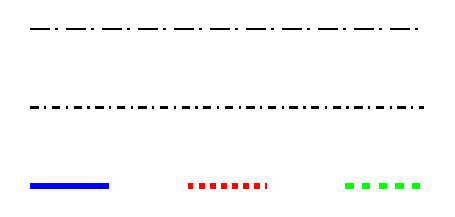
\begin{tikzpicture}
    \draw[line width=2pt, blue] (0,0) -- (1,0);

    \draw[line width=2pt, red, dotted] (2,0) -- (3,0);

    \draw[line width=2pt, dashed, green] (4,0) -- (5,0);

    \draw [thick,dash dot] (0,1) -- (5,1);  
    \draw [thick,dash pattern={on 7pt off 2pt on 1pt off 3pt}] (0,2) -- (5,2);
\end{tikzpicture}

\bigskip

Drawing an arc

\lstinputlisting{tikz/arc.tex}

\medskip

\input{tikz/arc.tex}

\bigskip

Draw a function

\lstinputlisting{tikz/function.tex}

\medskip

\input{tikz/function.tex}

\bigskip

Drawing rectangles and moving objects

\lstinputlisting{tikz/rectangle.tex}

\medskip

\input{tikz/rectangle.tex}

\bigskip

%input text left right bottom top

\bigskip

Use of variables

\lstinputlisting{tikz/variable.tex}

\medskip

\input{tikz/variable.tex}

\bigskip

Use of points

\lstinputlisting{tikz/node.tex}

\medskip

\input{tikz/node.tex}

\bigskip

Use of nodes

\lstinputlisting{tikz/node3.tex}

\medskip

\input{tikz/node3.tex}

\bigskip

Use of nodes

\lstinputlisting{tikz/node2.tex}

\medskip

\input{tikz/node2.tex}
